\documentclass[12pt,thmsa]{article}\usepackage[]{graphicx}\usepackage[]{color}
% maxwidth is the original width if it is less than linewidth
% otherwise use linewidth (to make sure the graphics do not exceed the margin)
\makeatletter
\def\maxwidth{ %
  \ifdim\Gin@nat@width>\linewidth
    \linewidth
  \else
    \Gin@nat@width
  \fi
}
\makeatother

\definecolor{fgcolor}{rgb}{0.345, 0.345, 0.345}
\newcommand{\hlnum}[1]{\textcolor[rgb]{0.686,0.059,0.569}{#1}}%
\newcommand{\hlstr}[1]{\textcolor[rgb]{0.192,0.494,0.8}{#1}}%
\newcommand{\hlcom}[1]{\textcolor[rgb]{0.678,0.584,0.686}{\textit{#1}}}%
\newcommand{\hlopt}[1]{\textcolor[rgb]{0,0,0}{#1}}%
\newcommand{\hlstd}[1]{\textcolor[rgb]{0.345,0.345,0.345}{#1}}%
\newcommand{\hlkwa}[1]{\textcolor[rgb]{0.161,0.373,0.58}{\textbf{#1}}}%
\newcommand{\hlkwb}[1]{\textcolor[rgb]{0.69,0.353,0.396}{#1}}%
\newcommand{\hlkwc}[1]{\textcolor[rgb]{0.333,0.667,0.333}{#1}}%
\newcommand{\hlkwd}[1]{\textcolor[rgb]{0.737,0.353,0.396}{\textbf{#1}}}%
\let\hlipl\hlkwb

\usepackage{framed}
\makeatletter
\newenvironment{kframe}{%
 \def\at@end@of@kframe{}%
 \ifinner\ifhmode%
  \def\at@end@of@kframe{\end{minipage}}%
  \begin{minipage}{\columnwidth}%
 \fi\fi%
 \def\FrameCommand##1{\hskip\@totalleftmargin \hskip-\fboxsep
 \colorbox{shadecolor}{##1}\hskip-\fboxsep
     % There is no \\@totalrightmargin, so:
     \hskip-\linewidth \hskip-\@totalleftmargin \hskip\columnwidth}%
 \MakeFramed {\advance\hsize-\width
   \@totalleftmargin\z@ \linewidth\hsize
   \@setminipage}}%
 {\par\unskip\endMakeFramed%
 \at@end@of@kframe}
\makeatother

\definecolor{shadecolor}{rgb}{.97, .97, .97}
\definecolor{messagecolor}{rgb}{0, 0, 0}
\definecolor{warningcolor}{rgb}{1, 0, 1}
\definecolor{errorcolor}{rgb}{1, 0, 0}
\newenvironment{knitrout}{}{} % an empty environment to be redefined in TeX

\usepackage{alltt}
\usepackage[french,english]{babel}
\usepackage[ansinew]{inputenc}
\usepackage[T1,OT1]{fontenc}
\usepackage{graphicx}
\usepackage{amsmath,amssymb,listings}
\usepackage{alltt,algorithmic,algorithm}
\usepackage{multicol}
\usepackage{cite}
\usepackage{fancyhdr}
\usepackage{setspace}
\usepackage{array}
\usepackage{amsfonts}
\usepackage{latexsym}
\usepackage{epsf}
\usepackage{umlaute}
\usepackage{setspace}
\usepackage{amsthm}
\usepackage{enumerate}


\setlength{\textwidth}{160mm}
\setlength{\textheight}{230mm}
\setlength{\oddsidemargin}{-5mm}
\setlength{\topmargin}{-10mm}

% to get rid of the numbers in the bibliography:
\makeatletter
\def\@biblabel#1{}
\makeatother



\title{Assignement 2}
\IfFileExists{upquote.sty}{\usepackage{upquote}}{}
\begin{document}


\noindent \textsc{University of Geneva}     \hfill \textsc{Bachelor in Economics and Management} \\
\textbf{Probability 1}                      \hfill \textsc{Bachelor in International Relations} \\
Dr. Daniel \textsc{Flores Agreda}                 \hfill Spring 2021  \\
ASSIGNMENT 02                               \hfill



\noindent
\makebox[\linewidth]{\rule{\textwidth}{0.4pt}}\\[1.5ex]

\section*{Exercise 1}


1. Let $ A $, $ B $ and $ C $ be three sets as shown in the following Venn diagram.\\
\begin{figure}[h!]
\begin{center}
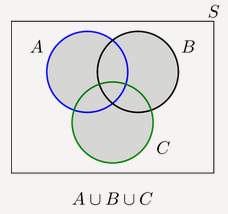
\includegraphics[scale=1]{Capture.png}
\end{center}
\end{figure}
\newline
For each of the following sets, draw a Venn diagram and shade the area representing the given set.
\begin{enumerate}[a)]
\item $ A \cup B \cup C $
\item $ A \cap B \cap C $
\item $ A \cup (B \cap C) $
\item $ A - (B \cap C) $
\item $ A \cup (B \cap C)^{c} $
\end{enumerate}
\vspace{1cm}
2. Using the Venn Diagrams, verify the following identities.
\begin{enumerate}[a)]
\item Transitive Property: If $A \subset B$ and $B \subset C$, then $A \subset C$. \\
\item Distributive Property: $A \cup (B \cap C) = (A \cup B) \cap (A \cup C)$, $A \cap (B \cup C) = (A \cap B) \cup (A \cap C) $ \\
\item De Morgan's Laws: $(A \cap B)^c = A^c \cup B^c $, $(A \cup B)^c = A^c \cap B^c $\\
\item $ A=(A \cap B) \cup (A-B) $
\item If $ A $ and $ B $ are finite sets, we have $ |A \cup B|=|A|+|B|-|A \cap B| $
\subitem Note that the symbol $ | . | $ indicates the cardinality, i.e. the measure of the ``number of elements of the set".
\end{enumerate}

\vspace{1cm}
3. Determine whether each of the following sets is countable or uncountable:
\begin{enumerate}[a)]
\item $ A=\{(x,y)|x \in N, y \in Z\} $
\item $ B=(0, 0.1] $
\item $ C=\{\frac{1}{n}|n \in N\} $
\item $ D=\mathbb{Q} $
\end{enumerate}


\section*{Exercise 2}


We consider an urn with $N$ marbles containing $r$ reds and $N-r$ blacks. We draw $n$ marbles randomly without repetition.
\begin{enumerate}
  \item How many possible cases (more properly, let us call them ``outcomes'') do we have?
  \item How many of these outcomes would include $k$ red marbles.
  \item Denoting by $P\text{(choosing k red marbles)}$ the probability of choosing $k$ red marbles, use the formula:
  $$
  P\text{(choosing k red marbles)}=\dfrac{\text{number of outcomes including k red marbles}}{\text{number of possible outcomes}},
  $$ to deduce $P\text{(choosing k red marbles)}$.
\end{enumerate}



\section*{Exercise 3}
There are 3 pairs of shoes of different color in a drawer. We randomly draw 2 shoes without repetition;
determine the probability\footnote{To compute the probability for an event $E$, use the formula
$$
P(E)=\dfrac{\text{number of cases in E}}{\text{number of possible cases}}.
$$}
associated with each of the following events:

 \begin{center}
 \begin{tabular}{l}
 $A$ : `they belong to the same pair';  \\
 $B$ : `there is a right shoe and a left shoe'.
 \end{tabular}
 \end{center}

\section*{Exercise 4}
Let $A$ be a die whose faces display the values 2, 2, 4, 4, 9, 9.  Let $B$ be a die whose faces display the
values 1, 1, 6, 6, 8, 8. We roll the two dice.

\begin{enumerate}
\item Write all the possible cases---more properly, let us call them ``outcomes''.
\item What is the probability\footnote{Use the same formula as in footnote 1.} that the result of $A$ is greater than the result of $B$?
\item What is the probability\footnote{Use the same formula as in footnote 1.} that the sum of the two dice equals $10$?
\end{enumerate}


\section*{Exercise 5}
A cafeteria offers a three-course menu. We choose a main course, a starch and a
dessert. The possible choices are given below:

\begin{itemize}
\item `Main course': Chicken (C) or roast beef (B);
\item `Starch': Pasta (P) or rice (R) or potatoes (T);
\item `Dessert': Ice cream(I) or jelly (J) or apple pie (A) or peach pie (P).
\end{itemize}

A person chooses a dish from each category.
\begin{enumerate}
\item How many possible menus are there in the basic set?
\item Let $A$ be the event: `we choose ice cream'. How many menus are there in $A$?
\item Let $B$ be the event: `we choose the chicken'. How many menus are there in $B$?
\item Give all the possible menus of the event $A \cap B$.
\item Let $C$ be the event: `we choose rice'. How many menus are there in $C$?
\item It is assumed that a person randomly selects his menu by associating an equal probability with
all the options for each category. What is the probability that the chosen menu belongs to event $A$?
Answer the same questions for event $B$ and for event $C$.

\end{enumerate}

\section*{Exercise 6 (Optional)}
In this problem, you are given descriptions in words of certain events (e.g., at least one of the events A,B,C occurs). For each one of these descriptions, identify the correct symbolic description in terms of A, B, C from Events E1-E7 below. Also identify the correct description in terms of regions (i.e., subsets of the sample space $\Omega$) as depicted in the Venn diagram below. (For example, Region 1 is the part of A outside of B and C.)
\begin{center}
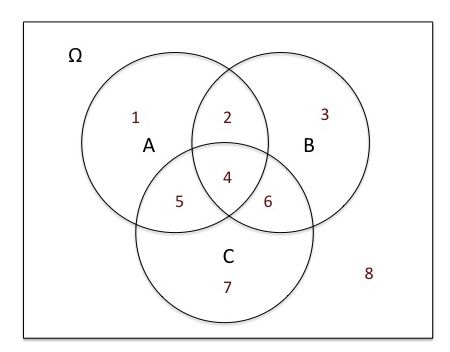
\includegraphics[width = 2in]{images1.jpg}
\end{center}

\noindent Symbolic descriptions: \\
Event E1: $A \cap B \cap C$ \\
Event E2: $(A\cap B \cap C)^c $ \\
Event E3: $ A \cap B \cap C^c $ \\
Event E4: $B \cup (B^c \cap C^c)$ \\
Event E5: $A^c \cap B^c \cap C^c $ \\
Event E6: $(A \cap B) \cup (A \cap C) \cup (B \cap C)$ \\
Event E7: $(A \cap B^c \cap C^c) \cup (A^c \cap B \cap C^c) \cup (A^c \cap B^c \cap C) $

\noindent Which Event or Regions satisfy the following conditions. \\
1. At least two of the events A, B, C occur. \\
2. At most two of the events A, B, C occur. \\
3. None of the events A, B, C occurs. \\
4. All three events A, B, C occur. \\
5. Exactly one of the events A, B, C occurs.\\
6. Events A and B occur, but C does not occur. \\
7. Either event B occurs or, if not, then C also does not occur.





\section*{Exercise 7 (Optional)}

A,B and C take turns flipping a coin, that is: A flips first, then B, then C, then A and so on. The first one get a head wins.
\begin{enumerate}
  \item Define the sample space $S$ of all the possible outcomes.
  \item Define the following events in terms of $S$:
\begin{enumerate}
  \item The event $A$: A wins.
  \item The event $B$: B wins.
  \item $(A \cup B)^c$
\end{enumerate}
\end{enumerate}

\iffalse
\section*{Exercise 3}

Let $\Omega$ be some set with at least one subset $A \subset \Omega$ and denote by $\emptyset$ the empty set. Show that the following sets are sigma-algebra:
\begin{enumerate}
  \item $\{\emptyset,\Omega\}$
  \item $\{\emptyset,A,A^c,\Omega\}$
\end{enumerate}
\fi

\end{document}




